\documentclass[UTF8, a4paper, 12pt]{ctexart}

% 基础包
\usepackage{amsmath}
\usepackage{amssymb}
\usepackage{enumitem}
\usepackage{booktabs}
\usepackage{tabularx}
\usepackage{graphicx}
\usepackage{geometry}
\usepackage{float}
\usepackage{hyperref}

% 代码高亮
\usepackage{listings}
\usepackage{xcolor}

% 页面设置
\geometry{
    left=2.5cm,
    right=2.5cm,
    top=2.5cm,
    bottom=2.5cm
}

% 代码样式设置
\lstset{
    basicstyle=\ttfamily\small,
    breaklines=true,
    showstringspaces=false,
    commentstyle=\color{gray},
    keywordstyle=\color{blue},
    stringstyle=\color{red},
    frame=single,
    numbers=left,
    numberstyle=\tiny\color{gray}
}

% 超链接设置
\hypersetup{
    colorlinks=true,
    linkcolor=blue,
    filecolor=magenta,      
    urlcolor=cyan,
    citecolor=green
}

\begin{document}


\section{图片格式支持测试}


本文档用于测试 MD2LaTeX 改进版对不同图片格式的支持能力。


\subsection{支持的图片格式测试}


\subsubsection{1. JPEG 格式图片}


JPEG 是最常用的图片格式,支持有损压缩,适合照片。


\begin{figure}[H]
    \centering
    \includegraphics[width=0.8\textwidth]{../../tests/images/test_image.jpg}
    \caption{JPEG 测试图片}
    \label{fig:jpeg_____}
\end{figure}



\subsubsection{2. PNG 格式图片}


PNG 支持无损压缩和透明度,适合图标和截图。


\begin{figure}[H]
    \centering
    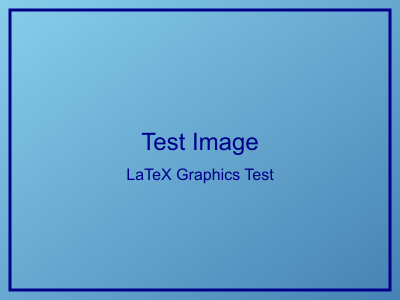
\includegraphics[width=0.8\textwidth]{../../tests/images/test_image.png}
    \caption{PNG 测试图片}
    \label{fig:png_____}
\end{figure}



\subsubsection{3. BMP 格式图片}


BMP 是 Windows 位图格式,通常文件较大但兼容性好。


% 图片格式提示: BMP格式可能需要转换为PNG
\begin{figure}[H]
    \centering
    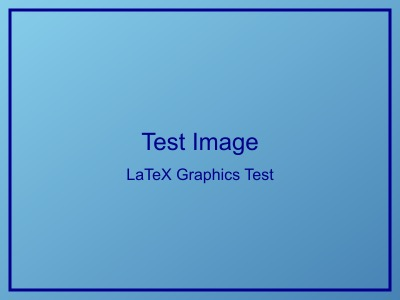
\includegraphics[width=0.8\textwidth]{../../tests/images/test_image.bmp}
    \caption{BMP 测试图片}
    \label{fig:bmp_____}
\end{figure}



\subsubsection{4. TIFF 格式图片}


TIFF 是高质量的图片格式,常用于印刷和专业图像处理。


% 图片格式提示: TIFF格式可能需要转换为PNG
\begin{figure}[H]
    \centering
    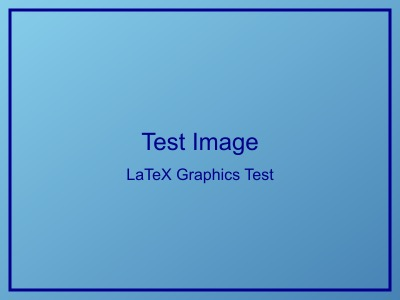
\includegraphics[width=0.8\textwidth]{../../tests/images/test_image.tiff}
    \caption{TIFF 测试图片}
    \label{fig:tiff_____}
\end{figure}



\subsection{图片处理功能测试}


\subsubsection{相对路径测试}


上面的图片都使用了相对路径 \texttt{../images/filename},测试路径解析功能。


\subsubsection{图片标题和说明}


每个图片都有描述性的 alt 文本,这将成为 LaTeX 中的 caption。


\subsubsection{LaTeX 图片环境}


生成的 LaTeX 代码应该包含:

\subsection{预期结果}


\subsubsection{LaTeX 输出}

每个图片应该生成类似以下的 LaTeX 代码:


\begin{lstlisting}[language=TeX, basicstyle=\ttfamily\small, breaklines=true]
\begin{figure}[H]
    \centering
    \includegraphics[width=0.8\textwidth]{../images/test_image.jpg}
    \caption{JPEG 测试图片}
    \label{fig:jpeg_测试图片}
\end{figure}

\end{lstlisting}


\subsubsection{PDF 编译}

\subsection{注意事项}


\subsection{测试目标}



\end{document}
